\documentclass{article}
\usepackage{color}
\usepackage{xcolor}
\usepackage{amsmath}
\usepackage[T1]{fontenc} 
\usepackage{tikz}

\begin{document}

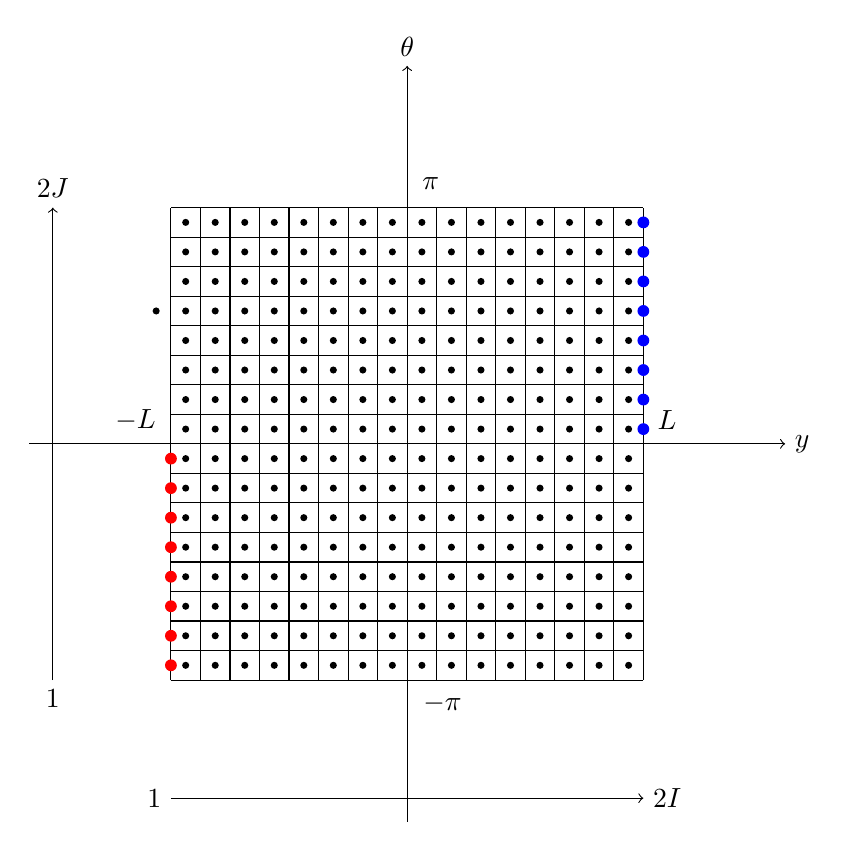
\begin{tikzpicture}[scale=1.5]
	\draw[step=0.25] (-2,-2) grid (2,2);
	\draw[->] (-3.2,0) -- (3.2,0) node[right] {$y$};
	\draw[->] (0,-3.2) -- (0,3.2) node[above] {$\theta$};
	\node at (-2.3,0.2) {$-L$};
	\node at (2.2,0.2) {$L$};
	\node at (0.2,2.2) {$\pi$};
	\node at (0.3,-2.2) {$-\pi$};

	\fill (-2.125,1.125) circle (.03);
	\foreach \i in {1,2,...,16} {
		\foreach \j in {1,2,...,16} {
			\fill (-2.125+0.25*\i,-2.125+0.25*\j) circle (.03) ;
		}
	}    
	\foreach \j in {1,2,...,8} {
		\fill[blue] (2,-0.125+0.25*\j) circle (.05) ;
		\fill[red] (-2,-2.125+0.25*\j) circle (.05) ; 
	}

	\draw[->] (-2,-3) node [left] {$1$} -- (2,-3) node[right] {$2I$};
	\draw[->] (-3,-2) node [below] {$1$} -- (-3,2) node[above] {$2J$};
\end{tikzpicture}

\end{document}